\subsection{Generalization across Deep Neural Networks}
In the previous experiments, expecially for what concerns Algorithm \ref{decentralized} which produced the best perturbations, we showed a remarkable generalization property of the universal avdersarial attacks: perturbations that have been generated starting from just a small portion of the dataset (1000 images out of 10000) are able to fool new images with high efficacy.

Moreover, in \cite{A2} has been shown that Universal Avdersarial Perturbations are not only universal across images, but also generalize well across different deep neural network architectures. Therefore we implemented the AlexNet convolutional neural network and test it on the adversarial examples produced by considering the loss function of LeNet-5.

Since the version of AlexNet that we implemented requires in input mini-batches of 3-channel RGB normalized images of shape $32\times 32\times 3$, we had to apply a constant padding to the $28\times 28$ images of MNIST in order to obtain a shape of $32\times 32$. After normalization, we extended the dimension to $32\times 32\times 1$ and used the method \textit{repeat} from TensorFlow on the third axis to get the desired shape of $32\times 32\times 3$. 

On the original MNIST test set, AlexNet achieved an accuracy of 98,18\% which abruptly dropped to 32,95\% on the adversarial examples obtained by applying the 100 queries-perturbation generated by Algorithm \ref{decentralized}.

To understand the entity of the attack, note that AlexNet was able to get a 73,73\% of accuracy on the same images perturbed with random noise (Gaussian with mean 0 and standard deviation 0.3). Figure \ref{fig:gen} shows the difference between an adversarial and a noisy example.

\begin{figure}[h]
	\centering
	\begin{subfigure}[b]{0.15\textwidth}
		\centering
		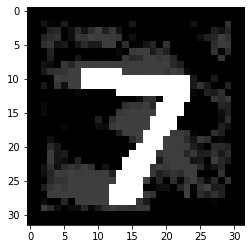
\includegraphics[width=2.5cm]{pert.png}
		\caption{}
	\end{subfigure}
	\hspace{0.7cm}
	\begin{subfigure}[b]{0.15\textwidth}
		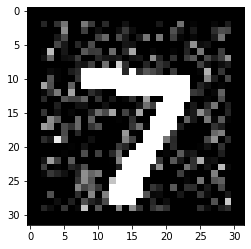
\includegraphics[width=2.5cm]{gauss.png}
		\caption{}
	\end{subfigure}
	\caption{{\small (a) Adversarial example. (b) Noisy example.\\ Note that the dataset preprocessing needed for the correct functioning of AlexNet, transformed the images in their negative colored version.}}
	\label{fig:gen}
\end{figure}